\subsubsection{Overdamped ($\Delta > 0$)}
This is the simplest and easiest case to deal with because our two roots, $r_1$ and $r_2$, are real and distinct. So, out solution is
\begin{equation*}
	y = C_1e^{r_1 t} + C_2e^{r_2 t}.
\end{equation*}
\begin{center}
	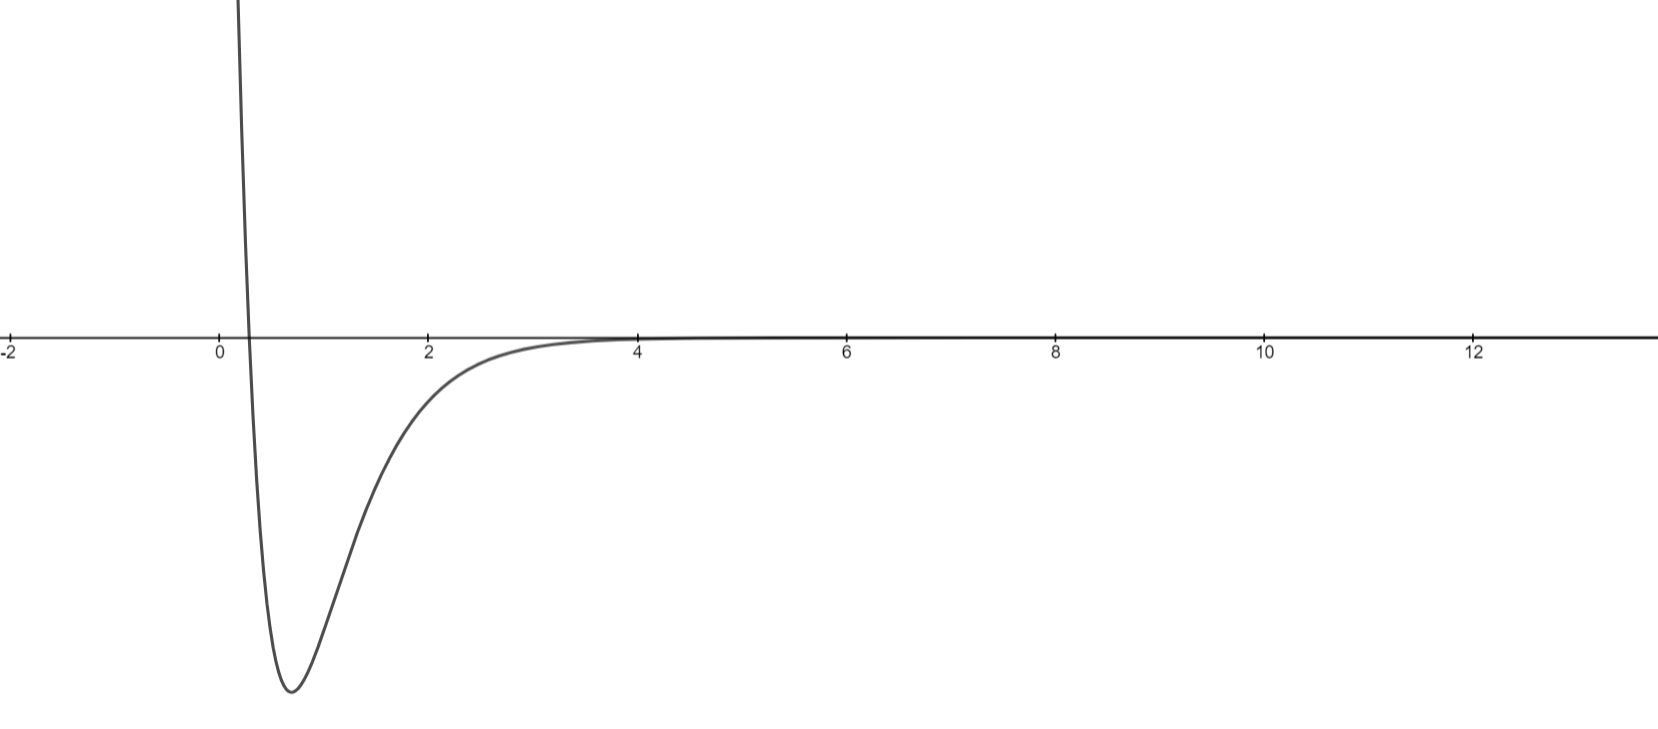
\includegraphics[width=0.5\textwidth]{./higherOrder/freeVibrs/overdamped.png}
\end{center}
We know that $r_1, r_2 < 0$, so
\begin{equation*}
	\lim\limits_{t \to 0}{C_1e^{r_1 t} + C_2e^{r_2 t}} = 0
\end{equation*}
meaning the mass's oscillation decays over time.